\section{Experimental QPI measurement}
Realspace \ac{QPI} signals are obtained by taking the grid map experiment on a region that presents \ac{QPI} patterns. In this section we will briefly explore \ac{QPI} measurement in the \ac{STM} experiment, more specifically, we will introduce the factors that dictate \ac{QPI} quality, discuss how to choose proper parameters that result in a good \ac{QPI} measurement, and finally we will present a specific challenge called the phase noise, which motivates our work in the next chapter.


\subsection{QPI measurement and quality}
As mentioned in Ch.2, taking a grid map is very involved. A successful grid map requires both an ideal instrumental setup and a set of proper measurement parameters based on the understanding of the targeting material. 

The key objective of an ideal instrumental setup is to create a stable environment and lower the system noise; as we discussed in Ch.2, this involves minimizing the noise from mechanical vibration, temperature fluctuation, and electronic instability of the system and maintaining a stable tip-surface tunneling junction. 

A grid map is defined by a $N\times N$ (assuming square) grid on a targeted area of $L \times L$ $nm^2$, this provides a spatial resolution $\Delta L = \frac{L}{N}$; In reciprocal space, this set up gives a range $Q = \frac{2 \pi}{\Delta L}$ with resolution $\Delta Q = \frac{2\pi}{L}$, the energy range and resolution is defined by the setting of the single-point spectroscopy performed on every grid point. 

A set of proper parameters for \ac{QPI} measurement aims to extract the most amount of information with the highest level of resolution given the constraints of the system. The most important constraint is the limiting cryogenic holding time. This puts a ceiling on the grid map run time, while different systems vary; typically, the cryogenic holding time is a fraction of a week. Within the boundary of the run time, we usually aim for a grid with a fine reciprocal resolution $\Delta Q$ and a reasonable reciprocal range $Q$, corresponding to a large field of view $L$ and a reasonable $\Delta L$. It is intuitive to have a proper size of reciprocal range $Q$ that is not infinitely large, as most of the q-space features reside within the Bragg peaks, exemplified by Fig. \ref{fig:ch5_ldos} c). But we also do not want the field of view $L$ to be too large, this is because in real experiments with finite noise level, the featured \ac{QPI} pattern has a finite lifetime and its intensity will dive under the noise at some cutoff distance $r_{cutoff}$ from the defect center; Thus, a field of view larger than the cutoff distance will instead decrease the signal to noise ratio. We illustrate cutoff distances in systems with different noise levels in Fig. \ref{fig:ch5_cutoff}. The noise level is set to be noiseless, SNR = 10, and SNR = 1.2, respectively; given the noise level shown in the green dotted line, we identify the furthest signal peak higher than the noise level and place a blue vertical line there. These vertical lines indicate the cutoff distances; and we can see with increasing noise level, $r_{cutoff}$ drops, and thus the optimal field of view should also drop.  

\begin{figure}
	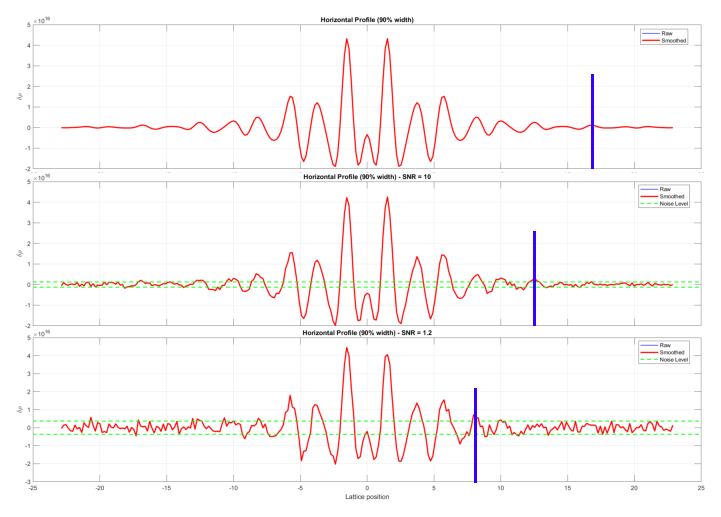
\includegraphics[width=\textwidth]{Ch5_fieldofview.pdf} 
	\centering
	\caption{Cutoff distances of QPI patterns with different signal-to-noise ratios. Three Horizontal Line profiles on $\delta\rho(\textbf{x}, E=0.45eV)$ with the noise of various levels. a) has no noise applied; b), c) have Gaussian noises applied with SNR = 10 and 1.2, respectively. Here the signal strength is defined as the variance of the noiseless $\delta\rho(\textbf{x}, E=0.45eV)$, see a) of Fig. \ref{fig:ch5_single_scattering}.}
	\label{fig:ch5_cutoff}
\end{figure}


\subsection{multi-defect QPI pattern and phase noise}
\ac{QPI} patterns present themselves around defects. While an ideal \ac{QPI} measurement is performed on isolated defects in a large field of view, it is normally difficult to find such a case. In real experiments, grid maps are usually taken on areas with multiple defects; this causes interference between the \ac{QPI} patterns originating from different defects, as hinted by Ch.5.2.4 when discussing Fig. \ref{fig:ch5_multi_scattering}.

This is problematic when we try to interpret the \textbf{q}-space \ac{QPI} map. As illustrated in Fig. \ref{fig:ch5_phasenoise}, when we have multiple defects scattered in the field of view, we start to see some noise patterns associated with the spatial distribution of the defects, as we can see by comparing c) and e), we see that with nothing but the relative locations of the defects changed, the corresponding \textbf{q}-space \ac{QPI} maps possess different noise patterns. This effect is called phase noise; it hinders our ability to analyze the underlying quasiparticle scattering process. 

\begin{figure}
	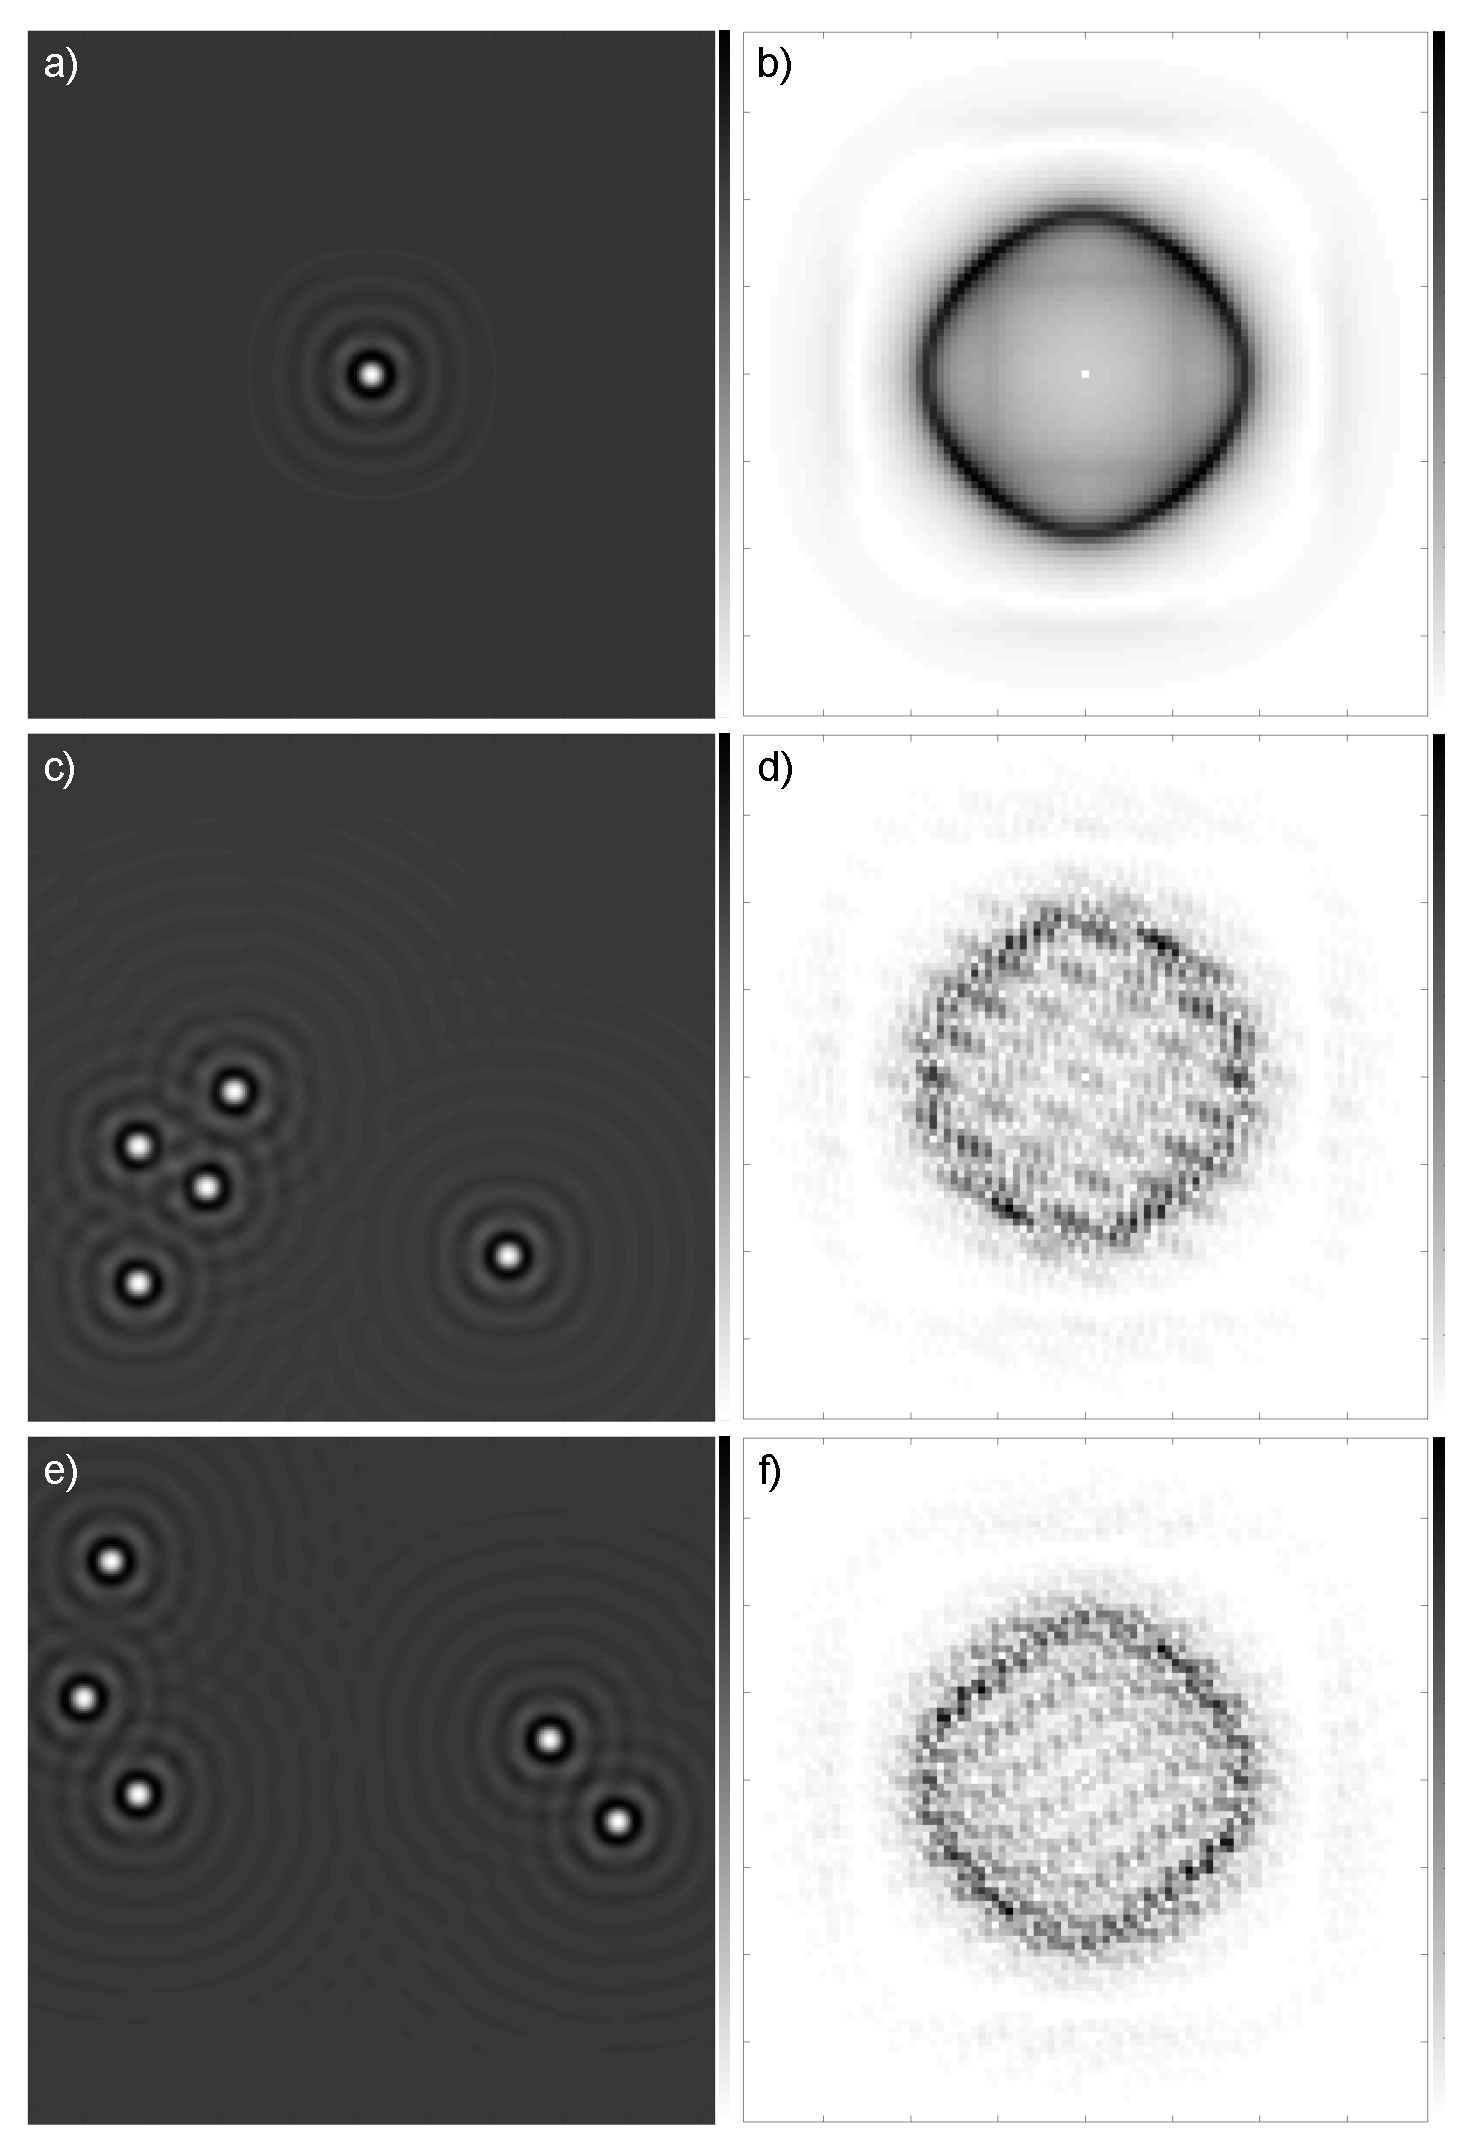
\includegraphics[width=0.8 \textwidth]{Ch5_phasenoise.pdf} 
	\centering
	\caption{Phase noise illustration. a),b): single defect scattering pattern and corresponding \textbf{q}-space QPI map. c)-f): multi-defect scattering with the same number of defects with different distributions, the corresponding QPI map presents phase noise with different patterns that associate with the defect distribution}
	\label{fig:ch5_phasenoise}
\end{figure}

Beyond the phenomenological illustration, we can further understand the source of phase noise with a mathematical analysis on multi-defect $\delta\rho(\textbf{x},\omega)$. We first discuss the form of the multi-defect T-matrix T, which is a $N_d \times N_d$ square matrix with entry T$_{\alpha \beta}$ representing the cross scattering term between defect m and n. We then separate the diagonal and off-diagonal terms and express T as\cite{leonard1972}:
\begin{align}
	\ T_{\alpha\beta} &= t_{\alpha} \delta_{\alpha\beta} + t_{\alpha} G_{0\alpha\beta} (1 - \delta_{\alpha\beta}) t_{\beta} + \sum_{\alpha' \neq \alpha, \beta} t_{\alpha} G_{0\alpha\alpha'} t_{\alpha'} G_{0\alpha'\beta} t_{\beta} + \cdots \label{eq_tmul}\\
	\label{eq.536}
	&= t_{\alpha} \delta_{\alpha\beta} + t_{\alpha} \sum_{\alpha'} \check{G}_{\alpha\alpha'} \ T_{\alpha'\beta},
\end{align}
\noindent where $t_{\alpha}$ is the T-matrix of a single impurity at site $\alpha$ and expressed on a matrix form in a localized basis set (i.e., expressed as the matrix with the same dimension as the multi-defect case but with only the $\alpha$'s diagonal entry none empty). And matrix $\check{G}_{\alpha\alpha'} = G_{0\alpha\alpha'}(1-\delta_{\alpha\alpha'})$, it contains the off-diagonal part of the Green's function. It has been shown by Fang et al. \cite{fangTheoryQuasiparticleInterference2013} that, in the Born approximation to the scattering amplitude, the first term dominates over the second term, and the latter can be omitted. We can, therefore, approximate multi-defect scattering with multiple single-defect scattering events. 

This approximation was then extended to the strong scattering case by Philipp et al. \cite{russmannInitioTheoryFourierTransformed2021}, under the assumption that the impurity concentration is low and the largest part of the surface is covered by pristine atoms and far from the impurities. They then utilized Equation \ref{eq.536} and further expressed the Green's function difference:

\[
\Delta G(\mathbf{r}, \mathbf{r}, E) = \int d^3 \mathbf{r}' \int d^3 \mathbf{r}'' \, G_0(\mathbf{r}, \mathbf{r}'; E) \, T(\mathbf{r}', \mathbf{r}''; E) \, G_0(\mathbf{r}'', \mathbf{r}; E)
\]

\begin{align}
	\label{eq.537}
	\Delta G_{\alpha \alpha} &= \Delta G^{(1)}_{\alpha \alpha} + \Delta G^{(2)}_{\alpha \alpha} \\
	\label{eq.538}
	&= \sum_{\alpha'} G_{0\alpha \alpha'} t G_{0\alpha' \alpha} + \sum_{\alpha'} G_{0\alpha \alpha'} t\sum_{\beta \beta'} \check{G}_{\alpha' \beta} \, T_{\beta \beta'} G_{0\beta' \alpha}.
\end{align}

\noindent By applying the stationary phase approximation \cite{lounisTheoryRealSpace2011} to $G_{0\beta'\alpha}$, and utilize the transnational symmetry of Bare lattice Green's function $G_0$, they showed:
\[
\Delta G^{(2)}_{\alpha\alpha}=\sum_{\alpha'}G_{0\alpha\alpha'}t\sum_{\beta\beta'}\check{G}_{\alpha'\beta}T_{\beta\beta'}K_{\beta'\alpha}e^{ik_{\beta'\alpha}\cdot R_{\beta'\alpha}},
\]
\noindent where the contribution of the last phase, $e^{ik_{\beta'\alpha}\cdot R_{\beta'\alpha}}$ can not be lifted, and is thus the source of the phase noise we observed in Fig. \ref{fig:ch5_phasenoise}. 

It is further noted that the contribution of the phase can be piratically canceled if we sum over all configurations of randomly distributed defects, which correspond to an infinitely large scanning surface, which can never be achieved. However, a decreased influence of this phase noise can be seen if we increase the density of the defects, as illustrated in Fig \ref{fig:ch5_changephasenoise}. This is because the patterns created by the phase noise become more fine-grained and can eventually be seen as featureless, similar to the random distribution of noise.  
%todo: verify whether this is true with more literature reviews. 

\begin{figure}
	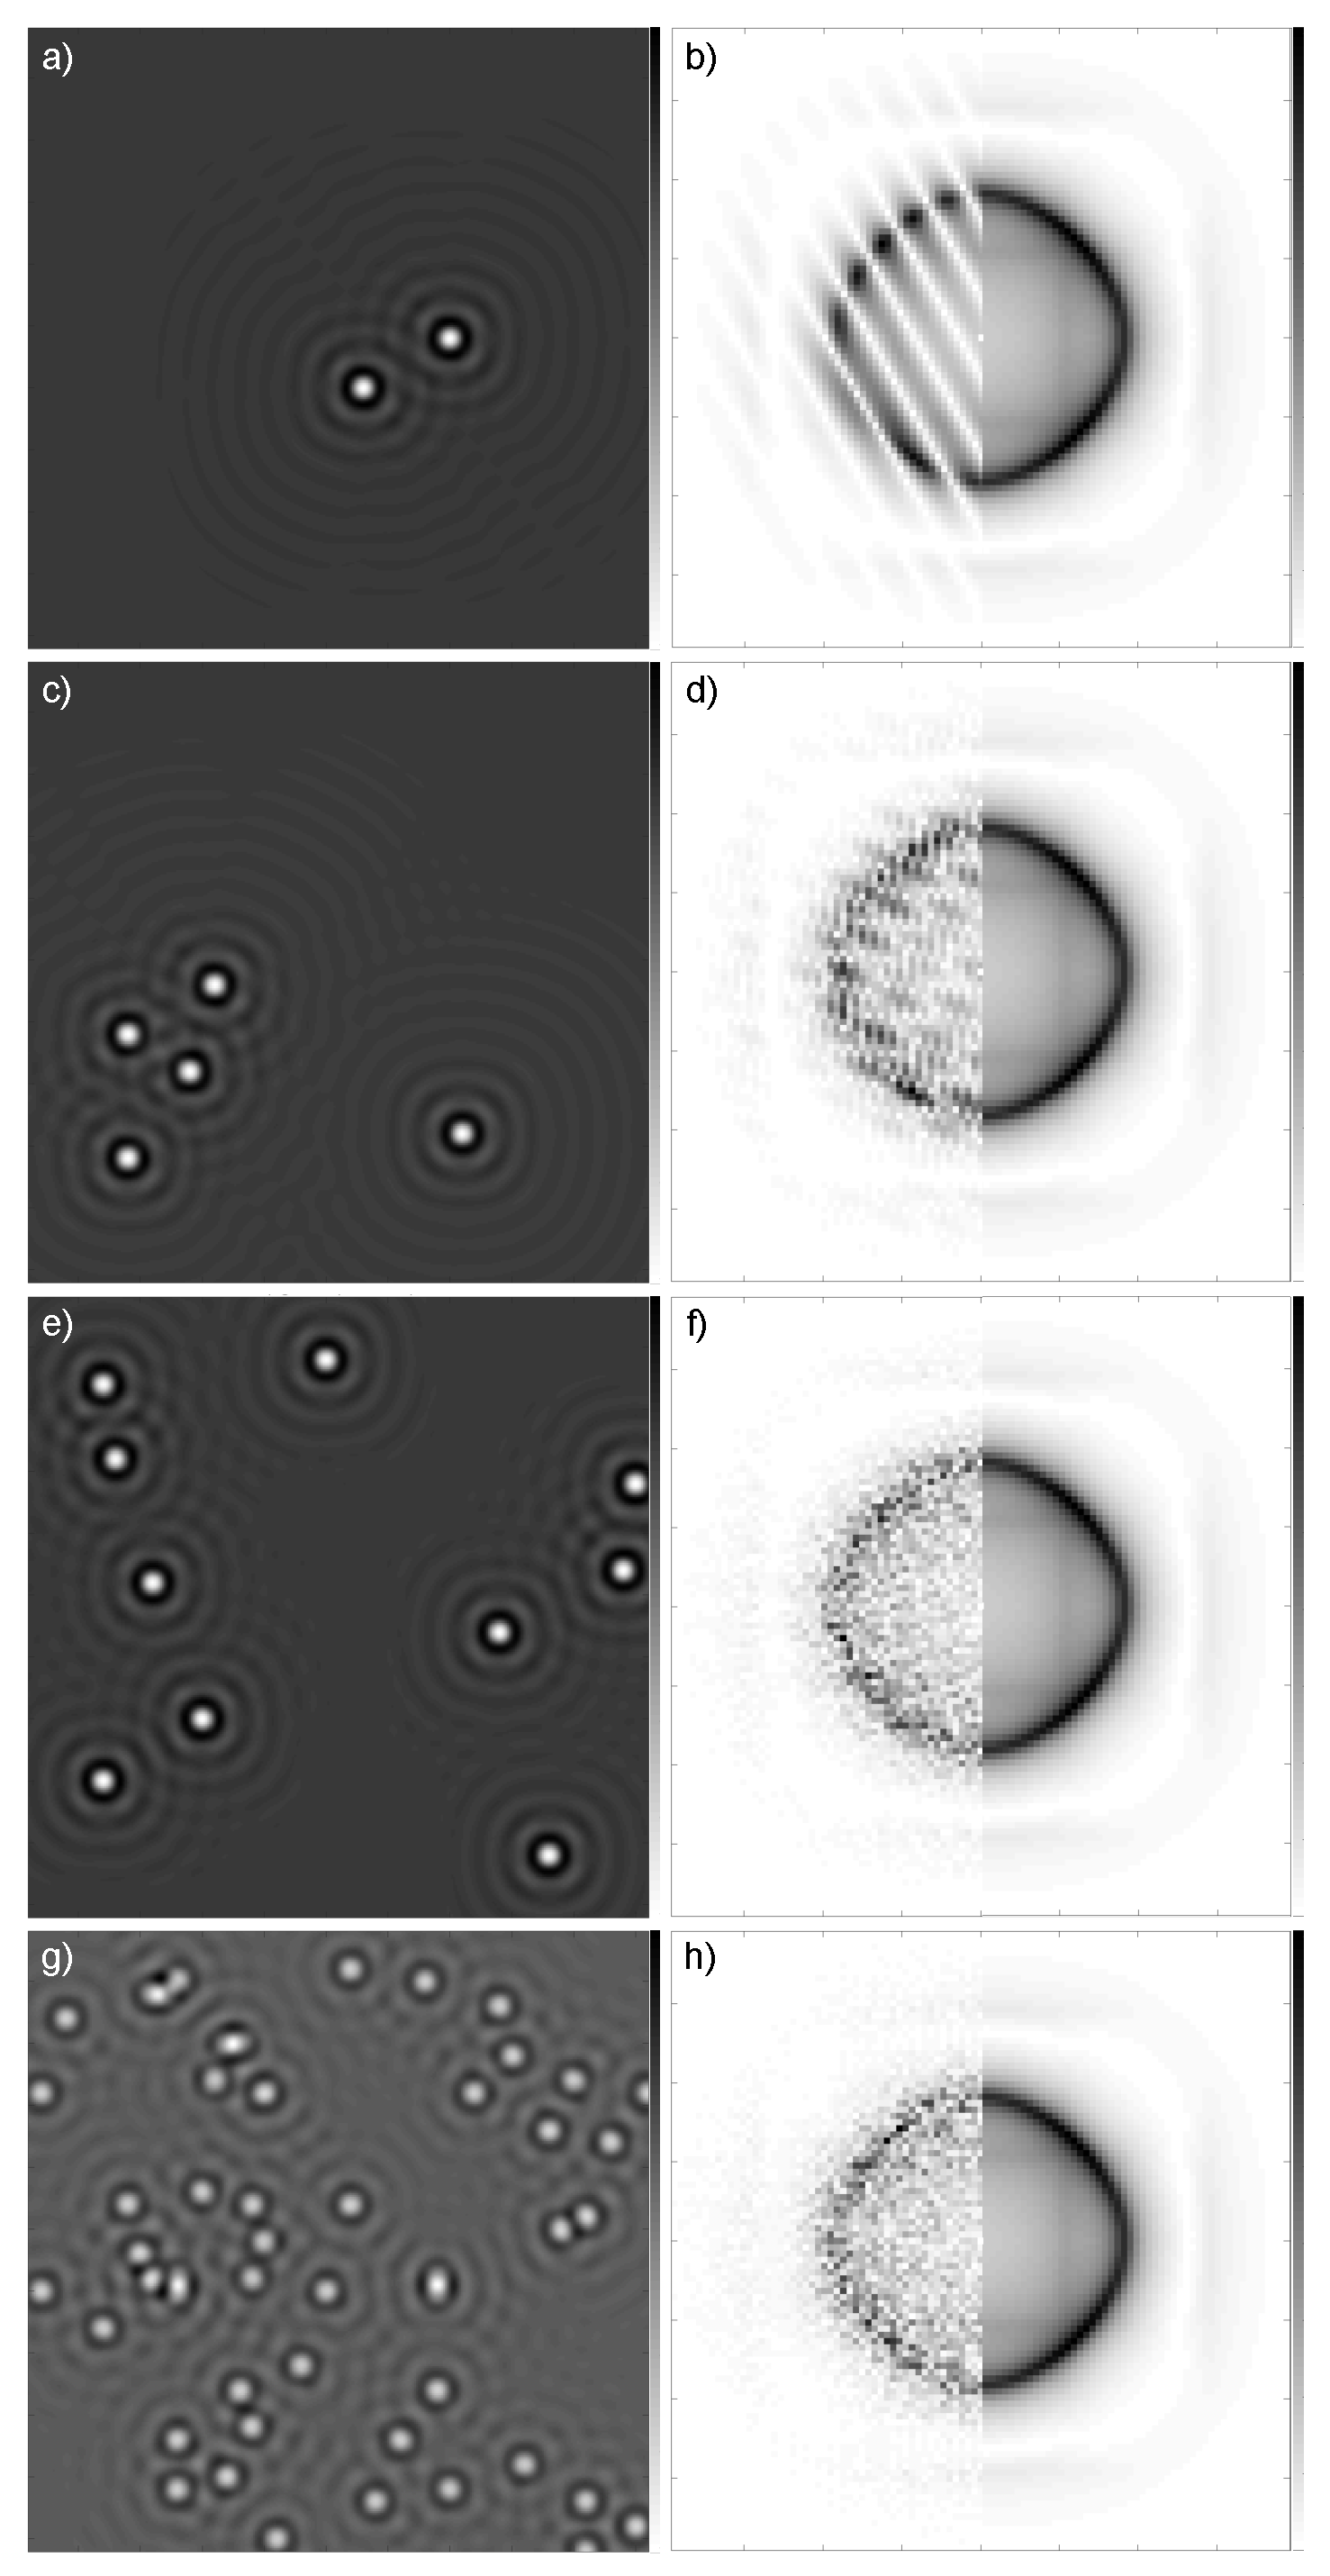
\includegraphics[width=0.8 \textwidth]{Ch5_changephasenoise.pdf} 
	\centering
	\caption{The effect of the phase noise is most prominent in the sparse defects regime. a)-h): $\delta\rho(\textbf{r},\omega)$ and \textbf{q}-space QPI plotted in pair with increasing defect concentration, showing the phase noise becomes more featureless. Single-defect QPI map is presented for reference on the right half of the \textbf{q}-space QPI.}
	\label{fig:ch5_changephasenoise}
\end{figure}